\chapter{Remote Work, Collaboration, and the Future Already Underway}

The interview begins with a familiar forecasting question: what are the three biggest technology trends over the next five to ten years? The answer, however, does not unfold as a clean list. It begins with a correction. Part of the future is already present, and the pandemic accelerated its arrival. What follows is therefore best read as a short causal lecture: remote work appears first, then the frame widens to collaboration, and finally the speaker explains why this mode of work became materially more practical than it used to be.

\section{A Forecast That Starts in the Present}

The opening question points forward, but the first move of the answer points backward and outward at once. We are told that some of the relevant shift has already happened, and that the pandemic accelerated it. In compact form, the first claim can be written as
\begin{equation}
A_{\mathrm{remote},\mathrm{post}} > A_{\mathrm{remote},\mathrm{pre}} .
\end{equation}
Here \(A_{\mathrm{remote}}\) denotes the adoption or practical intensity of remote work. The inequality is qualitative, not statistical. Its role is simply to preserve the speaker's order of thought: before we speculate about the future, we notice that one important transition is already underway.

This is an important narrative move. The answer is not really saying, ``Let me guess what comes next.'' It is saying, ``Let us notice what has already crossed from possibility into normal practice.''

\section{Remote Work and the Deeper Category}

The first named trend is remote work. But the answer does not stop there. It immediately widens: not only remote work, but any type of collaboration. That broadening matters. Remote work is the visible social form; collaboration is the deeper operating mechanism.

To keep the discussion organized, let us introduce a cautious notation:
\begin{itemize}
\item \(B\): effective internet access speed or bandwidth,
\item \(C\): the capability and maturity of collaboration tools,
\item \(V_{\mathrm{remote}}\): the practical viability of remote work.
\end{itemize}
With that notation, the speaker's broad point can be summarized by the monotone relation
\begin{equation}
V_{\mathrm{remote}} = f(B,C),
\qquad
\frac{\partial V_{\mathrm{remote}}}{\partial B} > 0,
\qquad
\frac{\partial V_{\mathrm{remote}}}{\partial C} > 0 .
\end{equation}
No precise functional form is asserted in the interview. The point is only that better connectivity and better collaborative tooling make distributed work more feasible. We begin with remote work because it is the most visible phenomenon, but the logic of the answer tells us that collaboration is the more fundamental category.

\section{Why This Changed}

At this stage the lecture raises its own natural question. If remote work and distributed collaboration are now so central, why were they not central earlier? The speaker answers by contrasting the present with the past: we did not previously have these tools in a sufficiently workable form.

\subsection{Question \& Answer}

\paragraph{Question.} Why is this way of working viable now when it was not viable before?

\paragraph{Answer.} Because the enabling layer improved. The speaker names two kinds of improvement: fast internet access speeds and collaborative tools. These do not merely decorate work; they change what kinds of work arrangements are practical.

A second compact inequality summarizes that claim:
\begin{equation}
P_{\mathrm{comm},\mathrm{now}} > P_{\mathrm{comm},\mathrm{past}} ,
\end{equation}
where \(P_{\mathrm{comm}}\) denotes the practical productivity of the communication and collaboration stack.

We can now write the logic of the answer as a short qualitative derivation:
\begin{align}
B_{\mathrm{now}} &> B_{\mathrm{past}},\\
C_{\mathrm{now}} &> C_{\mathrm{past}},\\
V_{\mathrm{remote}}(B_{\mathrm{now}},C_{\mathrm{now}})
&>
V_{\mathrm{remote}}(B_{\mathrm{past}},C_{\mathrm{past}}),\\
A_{\mathrm{remote},\mathrm{now}}
&>
A_{\mathrm{remote},\mathrm{past}} .
\end{align}
The last line should not be read as a theorem proved from data inside the interview. It is the speaker's practical conclusion: once connectivity and coordination improve enough, remote work moves from being awkward and exceptional to being normal and productive.

Since this passage gives us no blackboard derivation, the right visual aid is a clean editorial reconstruction of the causal chain:

\begin{figure}
\centering
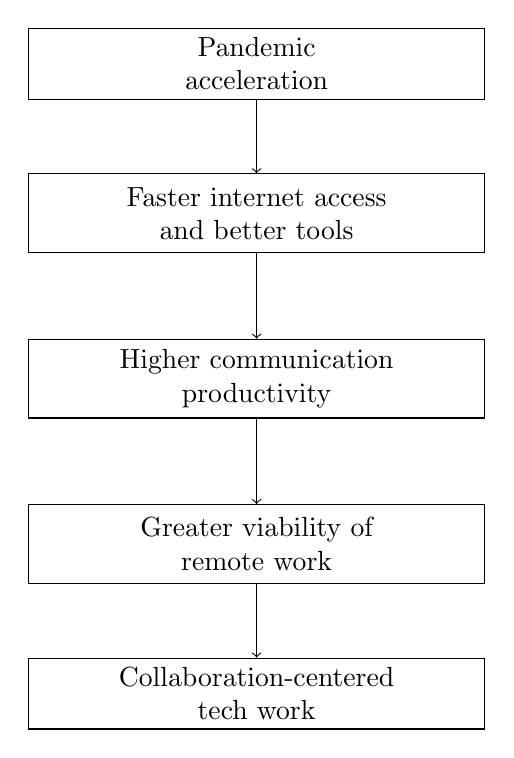
\begin{tikzpicture}[x=1cm,y=1cm]
\node[draw, rectangle, minimum width=5.8cm, minimum height=0.9cm, align=center] (a) at (0,0) {Pandemic\\acceleration};
\node[draw, rectangle, minimum width=5.8cm, minimum height=1.0cm, align=center] (b) at (0,-1.9) {Faster internet access\\and better tools};
\node[draw, rectangle, minimum width=5.8cm, minimum height=1.0cm, align=center] (c) at (0,-4.0) {Higher communication\\productivity};
\node[draw, rectangle, minimum width=5.8cm, minimum height=1.0cm, align=center] (d) at (0,-6.1) {Greater viability of\\remote work};
\node[draw, rectangle, minimum width=5.8cm, minimum height=0.9cm, align=center] (e) at (0,-8.0) {Collaboration-centered\\tech work};

\draw[->] (a.south) -- (b.north);
\draw[->] (b.south) -- (c.north);
\draw[->] (c.south) -- (d.north);
\draw[->] (d.south) -- (e.north);
\end{tikzpicture}
\end{figure}

The order of the boxes follows the spoken sequence closely. The pandemic is not treated as the deep cause of collaboration itself, but as the accelerator that pushed an already possible shift into broad adoption.

\section{Zoom, Slack, and Even Email}

The answer now moves from general mechanism to named examples: Zoom, Slack, and even email. This is a useful rhetorical step. The speaker is not offering a product ranking. He is grounding the abstract claim in ordinary tools that listeners already recognize.

We may collect those examples as
\begin{equation}
\mathcal{T}_{\mathrm{comm}}=\{\mathrm{Zoom},\mathrm{Slack},\mathrm{email}\}.
\end{equation}
Again, this set has a modest role. It is not a taxonomy of the entire market. It is a compact way to preserve the lecture's move from infrastructure and tool quality to concrete instruments of daily work.

\paragraph{Claim.} These tools have become much more productive than they used to be.

\paragraph{Mechanism.} Once communication tools become fast, stable, and easy to use, they no longer merely imitate in-person contact poorly. They begin to support real coordination, handoff, and continuing work across distance.

\paragraph{Consequence.} The future of tech work is described less by a single app than by a thicker collaborative environment in which distributed work becomes routine.

The mention of email is especially revealing. Zoom and Slack are obvious collaboration tools, but ``even email'' signals that the speaker is talking about the whole communication layer, not just the latest software category.

\section{Collaboration as the Deeper Trend}

The closing claim is sharp: collaboration is definitely the future for tech work, and remote work comes with it. We should preserve the order of emphasis. The deeper trend is not simply that people stay home. It is that technical work is increasingly organized through tools that make cooperation at a distance natural.

A final compressed chain captures that hierarchy:
\begin{equation}
C \uparrow \;\Rightarrow\; V_{\mathrm{remote}} \uparrow \;\Rightarrow\; A_{\mathrm{remote}} \uparrow .
\end{equation}
This is not meant as a full economic model. It is a faithful shorthand for the speaker's structure of reasoning. Better collaboration capability raises the feasibility of remote work, and once remote work becomes feasible, its adoption rises.

For entrepreneurship, the implication is concrete. A founder should not think only about where employees sit. We should think about the operating system of work itself: how information moves, how people coordinate, how tools reduce friction, and how a company becomes legible to itself even when its members are distributed.

\section{Summary}

The lecture begins with a question about three future trends, but this excerpt develops one central cluster of ideas. First, part of the future has already arrived. Second, the pandemic accelerated that shift. Third, remote work is the visible form of a deeper change, namely the rise of collaboration as the core operating principle of modern tech work. Fast internet access and better collaborative tools explain why this arrangement is now materially more productive than it used to be.

That is the passage's real spine. We start with a forecast, we pivot to an observed transition, we ask why it became viable, and we end with a hierarchy: collaboration first, remote work second.